\alg{Best Of Sampled Set}~\cite{asmuth09}, or \alg{BOSS}, is a Bayesian approach to model-based reinforcement learning. This algorithm makes use of a general prior to sample entire models from the posterior. It works by sampling a set of models and combining them (see Figure~\ref{sec:boss:hyper-model}) in a way that helps it choose the best in each situation.

This algorithm follows a strong tradition in model-based reinforcement learners of optimism in the face of uncertainty. One of the best-known model-based RL algorithms, \alg{RMAX}~\cite{brafman03}, approaches this idea by locking unknown states to the highest possible value, or $\Vmax$.

\section{Algorithm}

The \alg{BOSS} algorithm, outlined in Figure~\ref{boss:fig:boss-general}, makes use of repeated samples from a posterior to create a hyper-model that can be used for trading off exploration and exploitation.


\begin{figure}[t]
\begin{center}
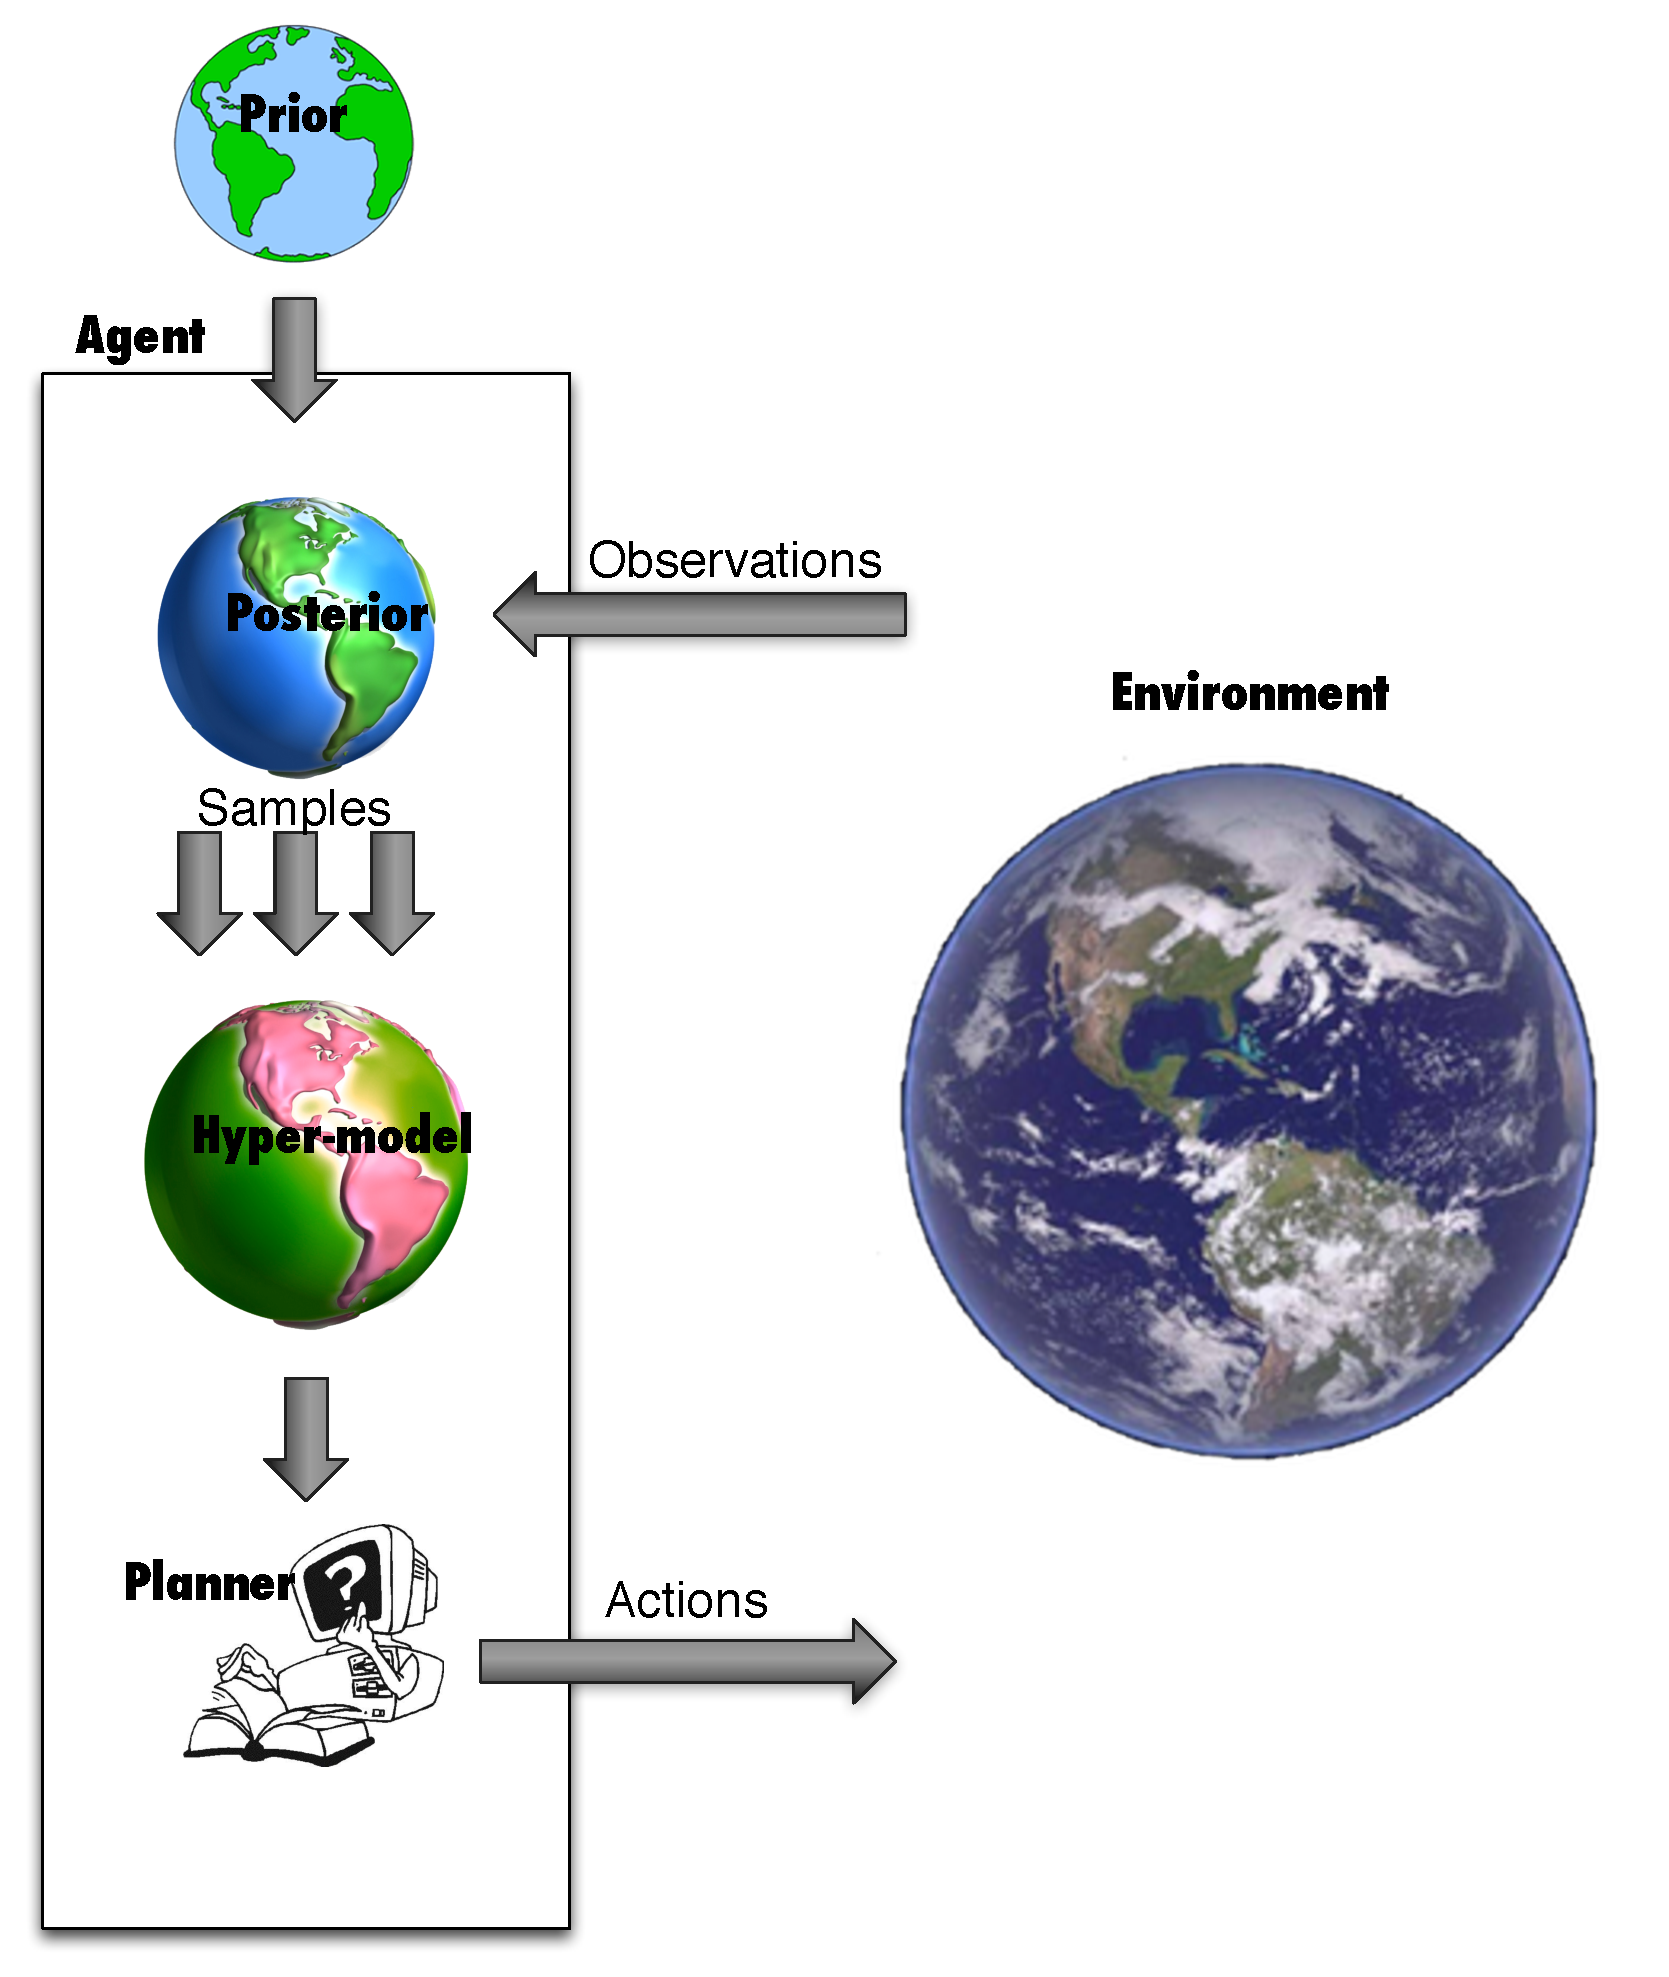
\includegraphics[width=0.75\linewidth]{boss-loop}
\caption{\alg{BOSS} combines observations made from the environment with the prior to create sets of posterior samples. These posterior samples are combined to create a hyper-model, which the planner takes as its model. The policy on the hyper-model is used in the environment.}
\label{boss:fig:boss-general}
\end{center}
\end{figure}

\begin{figure}[t]
\begin{center}
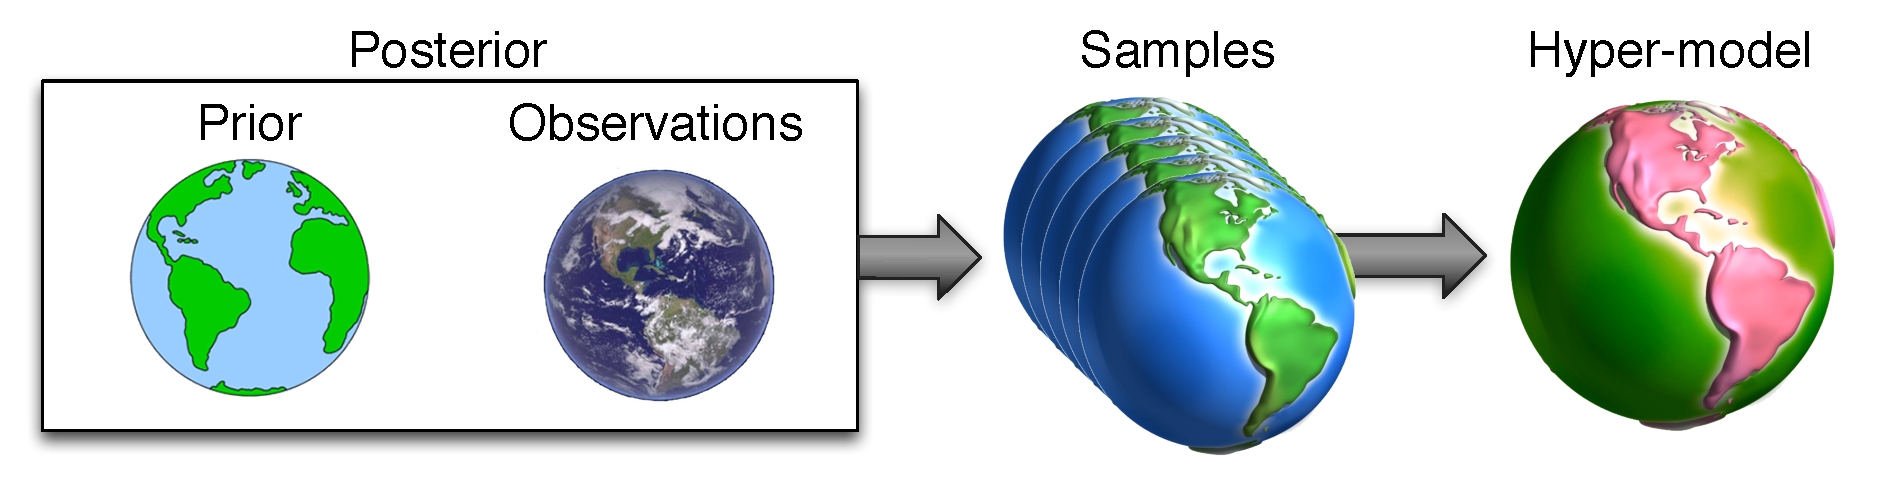
\includegraphics[width=0.9\linewidth]{hypermodels}
\caption{A posterior is created by combining the prior with observations made by the agent in the environment. Every the agent decides that it has learned something, several samples are drawn from the posterior and combined to create the hyper-model.}
\label{sec:boss:hyper-model}
\end{center}
\end{figure}



There are two distinct cases to which \alg{BOSS} algorithm can be analyzed: in general and for discrete action and state spaces. The general case, for arbitrary state and action spaces, works as an effective exploration heuristic, while the specific case has formal efficiency guarantees. We will discuss first the general case, and then the discrete state-action case.

\subsection{BOSS for general models} 

The \alg{BOSS} algorithm requires two important black boxes: a posterior sampler and a planner. 

It is important to remember that these two black boxes encapsulate entire fields of active and interesting research and should not be thought of as solved problems when designing an agent. However, using \alg{BOSS} as an exploration mechanism allows us to separate the reinforcement--learning problem from the planning and inference problems. This separation allows reinforcement--learning researchers to more easily draw on advances in other communities and to build on them.

\subsubsection{The posterior sampler}

The model posterior is the combination of a model prior (provided by the programmer) and observations (collected by the agent or provided by the environment). Techniques for deriving a posterior are covered in Chapter~\ref{sec:models}.

The posterior sampling black box must have the ability to sample from the set of worlds that are possible, given the observations made so far. The sampled model must be able to simulate transitions to next-states and rewards, given an action and the state it was taken from.

As the agent explores the world, taking actions and receiving feedback, it feeds the observations it has received to the posterior sampler. As the posterior sampler gets more and more data, the models sampled from it become more and more accurate, at least where the concentration of samples is high enough.

A posterior sampler can only be useful if some sort of accuracy guarantee is possible. That is, as more observations are made, models sampled from the posterior become closer to the truth, at least in the parts of the model associated with the observations. It is not always the case that a posterior will become more accurate with more data. A simple example is a prior that says that a coin will either always turn up heads or always turn up tails. The moment that both a head and tail have been observed, \reply{ the posterior becomes broken. The posterior distribution for the coin's bias,
\begin{eqnarray}
P(\rho|h=1,t=1) &=& \frac{\mbox{Bin}(H=1|\rho,n=2)P(\rho)}{P(H=1,n=2)}, \label{sec:boss:eqn:bad-flip}
\end{eqnarray}
is now undefined. The denominator in Equation~\ref{sec:boss:eqn:bad-flip} is zero, since the coin must be either two-headed or two-tailed.
}
For the general case, I will not specify exact accuracy guarantees. For the special case in Section~\ref{boss:alg:disc} there is a concrete assumption that must be met to guarantee efficiency.

\subsubsection{The planner}

\alg{BOSS} requires a planner that, given a model, can (probably) find an (approximately) optimal action for any given state. The specifics of how the planner comes to its decision, including the number of samples drawn from the model and how much time is spent in computation, are orthogonal to \alg{BOSS}'s goal of low exploration complexity.

Fortunately, since the planner's operation is orthogonal to how \alg{BOSS} works, the two can be analyzed separately.

Although the planner is decoupled from \alg{BOSS}'s operation, it is tied closely to the posterior sampler. More accurately, it is closely tied to the models generated by the posterior sampler. The planner must be able to work in whatever model the posterior sampler can create. More than that, it must be able to work in a hyper-model, created by melding some number of the posterior sampler's models together, as discussed in Section~\ref{boss:alg:gen:hyper}.

\subsubsection{Hyper-models}

\label{boss:alg:gen:hyper}

\begin{figure}[t]
\begin{center}
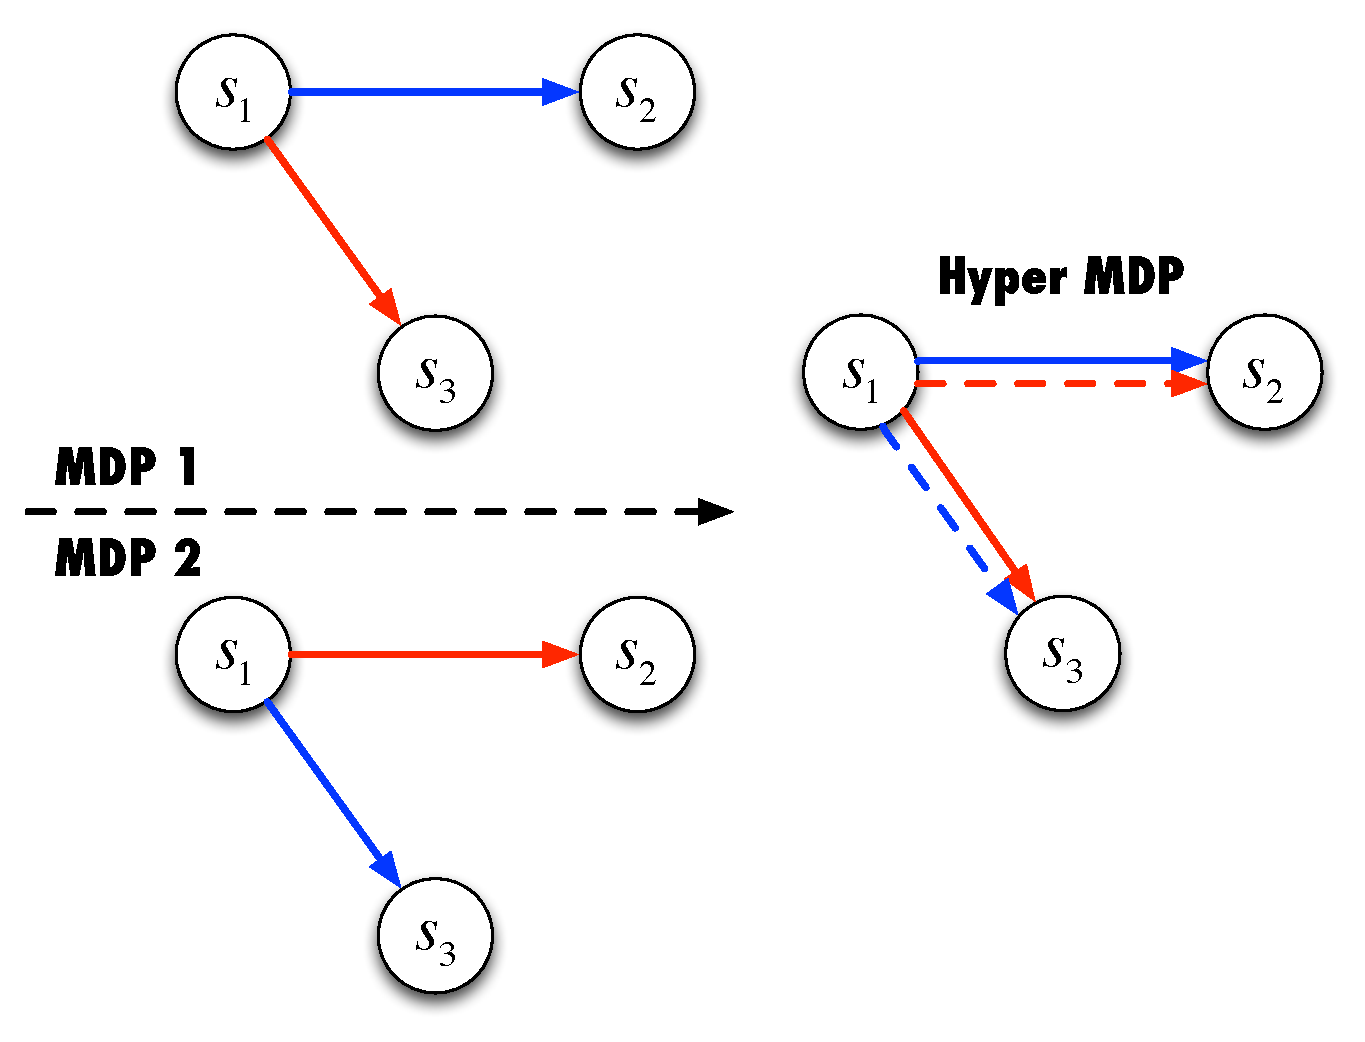
\includegraphics[width=0.45\linewidth]{hyper-construction}
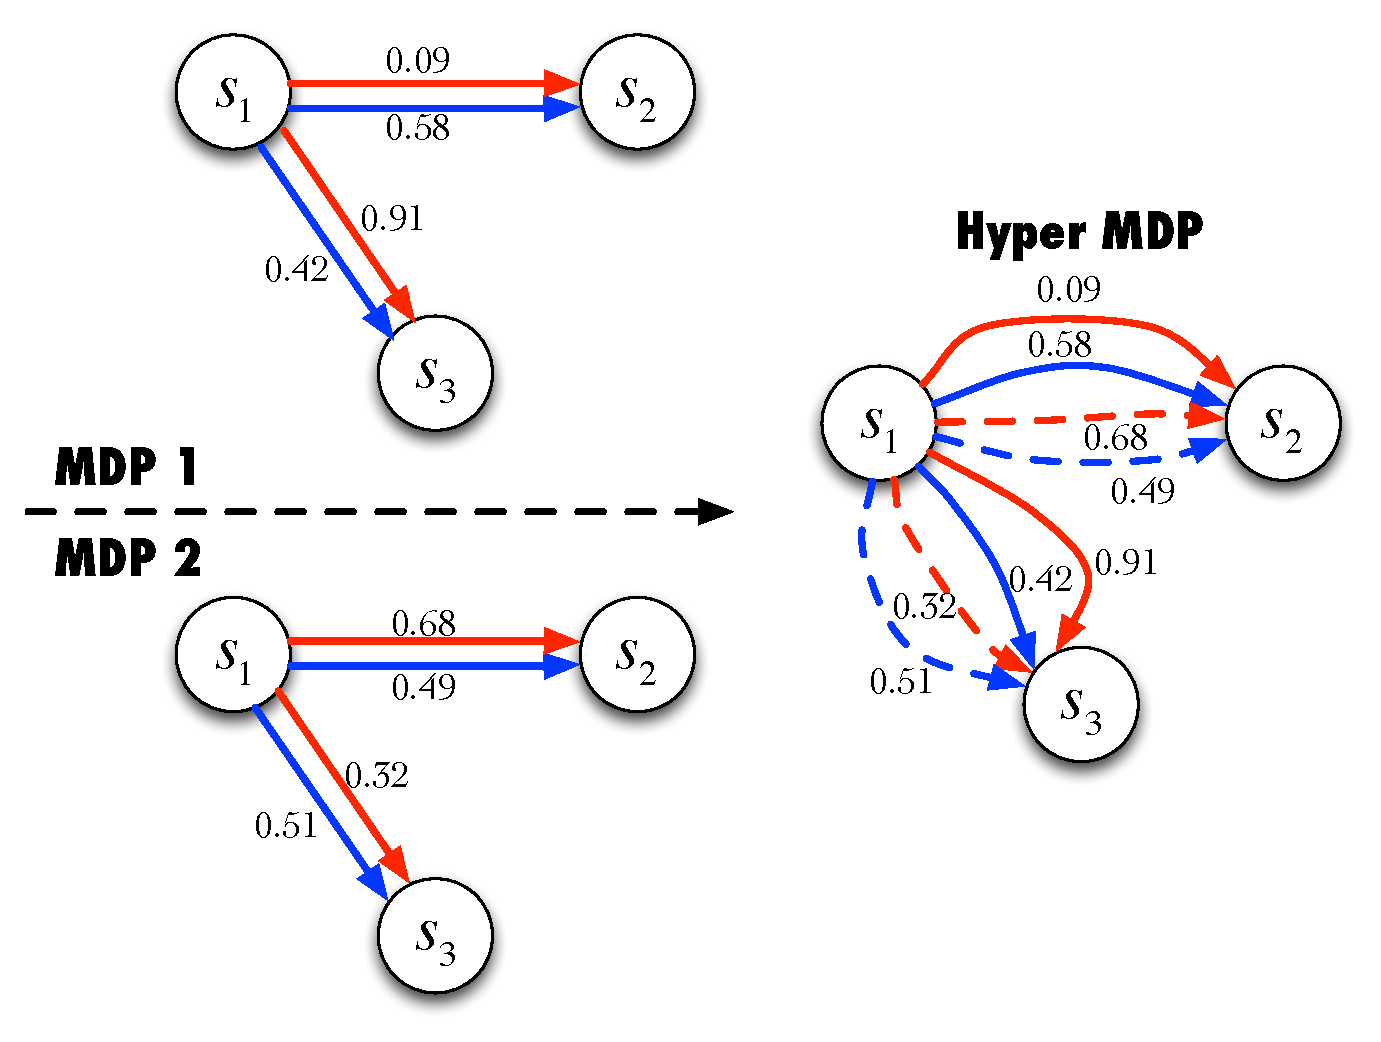
\includegraphics[width=0.45\linewidth]{hyper-stoch-construction}
\caption{\textbf{Left:} Two samples with the same state- and action-spaces and deterministic dynamics are combined to create a hyper-model. Every action from each of the provided models exists in the hyper-model. \textbf{Right:} Two stochastic MDPs are combined to create a stochastic hyper-model MDP. In both cases, solid lines in the hyper-model indicate the action was taken from the upper sample, and dashed lines indicate the action was taken from the lower sample.}
\label{sec:boss:hyper-model-creation}
\end{center}
\end{figure}


\begin{figure}[t]
\begin{center}
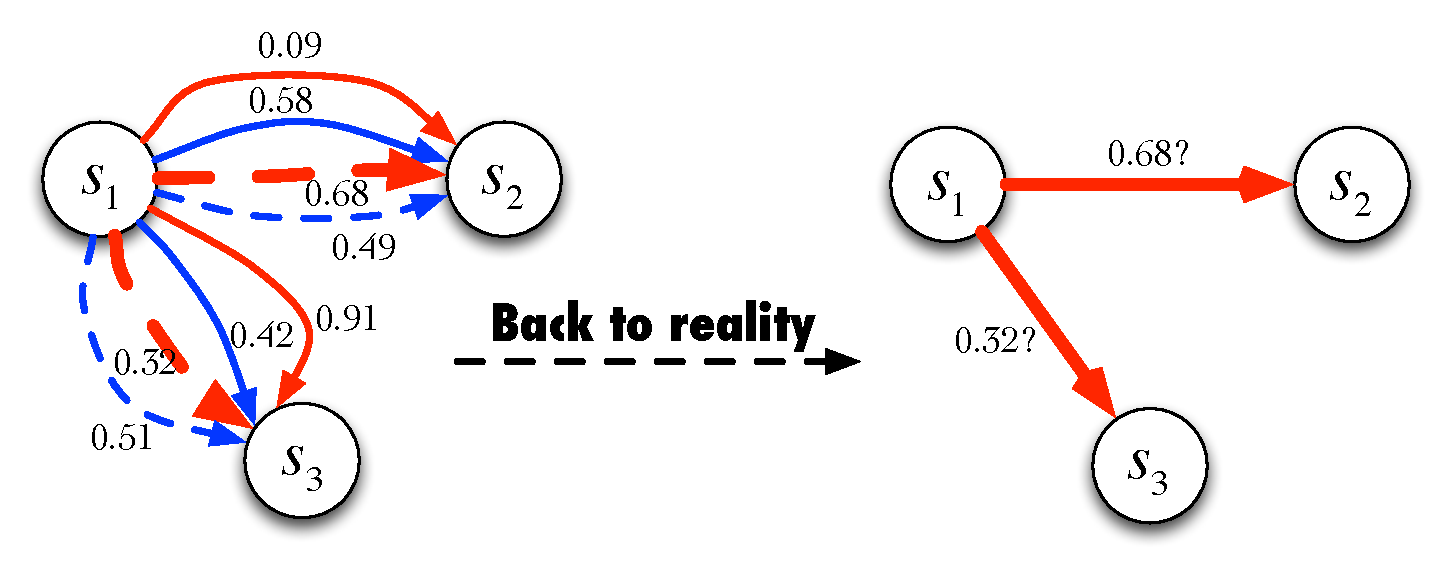
\includegraphics[width=0.75\linewidth]{hyper-to-real}
\caption{The agent chooses the best policy in the hyper-model, and then translates it back into the environment it is dealing with. In this case, it chose the red dashed action (perhaps $s_2$ has a higher value than $s_3$. In the real environment, the agent will choose the red action, hoping that it has a high probability of resulting in transition to $s_3$. If this hope is in error, the agent may try the action several times and eventually have enough evidence to effect a change in the posterior.}
\label{sec:boss:hyper-to-real}
\end{center}
\end{figure}

A hyper-model is the combination of some set of $K$ models with identical action and state spaces, but possibly differing dynamics (as in Figure~\ref{sec:boss:hyper-model-creation}). The resulting hyper-model \note{pp: How is the hyper-model constructed?  Be more precise.  Perhaps provide pseudocode.} has the same state space as each of its sub-models, but has one more feature in its action space. This feature, $k\in\{1,...,K\}$, indicates from which sub-model the dynamics of this action are taken. That is, the action $(2, a)$ has the same next-state and reward distributions that action $a$ has in model $2$.

\reply{
Formally, a hypermodel $m'$ can be constructed from $k$ MDPs $m_1, m_2, ... , m_k$ that have the same state-space $S$ and action-space $A$. They may each have unique transition and reward functions $T$ and $R$. The hypermodel $m'$ has state-space $S$ and action-space $A \times \{i|i\in \mathbb{N},i\geq 1, i\leq k\}$. The transition function for $m'$ is defined to be
\begin{eqnarray}
T_{m'}(s'|s,\langle a, i \rangle) &=& T_{m_i}(s'|s, a).
\end{eqnarray}
That is, the probability of ending up in state $s'$ after taking the action $\langle a, i\rangle$ is the same as the probability of ending up in state $s'$ when taking action $a$ in MDP $m_i$. Similarly, the reward function for $m'$ is defined to be
\begin{eqnarray}
R_{m'}(s,\langle a, i \rangle) &=& R_{m_i}(s, a).
\end{eqnarray}
}

Intuitively, an agent acting according to $m'$ is free to choose the dynamics from any of the sampled models during each step. An optimistic agent, one that thinks the best of the unknown, can choose the dynamics that give it the biggest advantage. This is an example of ``optimism in the face of uncertainty'', where the agent is drawn to parts of the state space that are either known to be good, or are not known. With this attack plan, the agent will either get good reward or get good knowledge. Since the amount of knowledge to be learned is usually finite, the agent will visit the unknown states enough to make them known, and be able to act without exploration in the future.

\alg{BOSS}'s method of model creation allows the hyper-model to retain all the optimism of any of its sub-models. The idea is that, for each state, at least one of the $K$ models will predict dynamics at least as good as the true model's dynamics.

The claim that the hyper-model is, for every state, at least as optimistic as any of its sub-models is detailed in Section~\ref{sec:boss:sub-model-optimism}.

It is important to choose $K$ carefully. A low value for $K$ will increase the odds that, for some set of $K$ models, there will be states for which \emph{no} model's dynamics will be as good as the true model's --- this situation breaks any guarantees that \alg{BOSS} offers. A high value for $K$ can cause two problems. First, the amount of work done by the planner increases, sometimes dramatically; the runtime complexity of most discrete-action planning algorithms relies linearly or super-linearly on the number of actions. Second, too much optimism can be a bad thing. In the extreme, as $K \rightarrow \infty$, all possible models will be represented in every set of $K$ sub-models. In this situation, the agent's observations have no effect on the hyper-model, since the likelihood of each sampled model is not taken into account when compositing the sub-models together. With a finite, yet large, $K$, the number of observations required to have a particular state's dynamics be accurate in each of the sub-models grows as a polynomial of $K$. While this growth rate doesn't make a dent in any theoretical guarantees, it does present serious issues in practice.

\subsubsection{Algorithm}

The basic \alg{BOSS} algorithm is as follows:
\begin{enumerate}
\item Sample $K$ sub-models from the posterior. \label{boss:alg:gen:step1}
\item Combine each of the $K$ models sampled into a hyper-model, as in Section~\ref{boss:alg:gen:hyper}.
\item Using the planner, act optimally according to the hyper-model until a discovery event occurs. \label{boss:alg:gen:step3}
\item Go back to Step~\ref{boss:alg:gen:step1}.
\end{enumerate}

This process is repeated forever, though eventually Step~\ref{boss:alg:gen:step3} will never complete, since the number of discovery events an agent can experience is bounded.

Here, we define a \emph{discovery event} to be an action taken that causes a state to go from unknown to known. How this change is quantified varies with the model and prior being used. As an example, with a discrete state and action space, a state may become known once each action has been attempted from that state some pre-determined number of times. In a continuous state space, reaching some action density at a state could be defined to trigger a discovery event.

A discovery event is a signal to the agent that the observations it has gathered have affected the posterior sufficently that the $K$ models it has been working with may now be out of date. A new hyper-model is created, from the new information, and the agent resumes its process of either getting high reward or making observations in states that are unknown (because they will have high reward in the hyper-model).

The agent will get high reward because states that are \emph{known} to be good will be accurately represented in each of the $K$ samples, and the planner will be using an accurate version of those states' dynamics when it plans, no matter which version of the action it chooses to use.

The agent will make observations in states that are \emph{unknown} because, for each unknown state, at least one of the $K$ sampled models will have dynamics that are optimistic for that state, making it more attractive to the agent than it would be otherwise.

\subsection{BOSS for discrete state and action spaces}
\label{boss:alg:disc}

With a discrete state and action space, where the model can be represented by an MDP, the \alg{BOSS} algorithm can be defined more exactly, and given formal efficiency guarantees.

\subsubsection{Knowness}

For any prior that supports (has a non-zero probability for) the true model, there will be some minimum number of observed transitions from a particular state, with a particular action, that is large enough to guarantee (with high probability) a posterior sample that is close to the truth for that state-action pair. We will call this threshold $B$. We choose $B$ such that after $B$ next-states have been observed for a particular state-action pair, with high probability the true next-state distribution is close to the distribution inferred from the observation set. The threshold $B$ is a function of the desired accuracy and probability of success.

A discovery event is then defined to occur on the $B^{\mbox{th}}$ transition from a particular state-action pair.

\section{Theoretical guarantees}

The \alg{BOSS} algorithm is both PAC-MDP and PAC-BAMDP, under slightly different conditions. The difference between optimal and Bayes-optimal, in this situation, hinges on whether the ``true'' MDP is \bed-learnable or the prior itself is \bed-learnable. This distinction is important to make, since with an especially strange prior, the posterior may not converge to something close to the true model after a reasonable number of observations. With this strange prior, \alg{BOSS} will still be PAC-BAMDP, but the Bayes-optimal and optimal policies may differ significantly.

\subsection{Definitions}

This section formalizes some definitions that are important for understanding the theorem and proof that follows.

\begin{defn}
\label{sec:boss:defn:local-opt}

An MDP $\hat m$ is said to be \emph{locally $\epsilon$-optimistic} at state-action pair $s, a$, with respect to a baseline MDP $m_0$, if
\begin{eqnarray}
R(s,a)+\gamma \sum_{s'} T_{\hat m}(s'|s,a) V_{m_0}(s')
&\geq&R(s,a)+\gamma \sum_{s'} T_{m_0}(s'|s,a) V_{m_0}(s') - \epsilon,
\end{eqnarray}
where $R$ is the reward function for MDP $m$, where $T_{m}$ is the transition function for MDP $m$, $V_m(s)$ is the value of state $s$ in MDP $m$.

That is, if the agent is able to take a single step from $s,a$ in $\hat m$, and then must exist in $m_0$ after that, it is able to achieve an expected discounted return that is at least as high as that that it could achieve starting in $m_0$, less $\epsilon$.

\end{defn}

\begin{defn}
\label{sec:boss:defn:local-acc}

An MDP $\hat m$ is said to be \emph{locally $\epsilon$-accurate} at state-action pair $s, a$, with respect to a baseline MDP $m_0$, if
\begin{eqnarray}
||T_{\hat m}(\cdot|s,a) - T_{m_0}(\cdot|s,a)||_\infty &\leq& \epsilon,
\end{eqnarray}
or
\begin{eqnarray}
\forall_{s'} \left|T_{\hat m}(s'|s,a) - T_{m_0}(s'|s,a)\right| &\leq& \epsilon,
\end{eqnarray}
where $T_{m}$ is the transition function for MDP $m$.

That is, the likelihood of ending up in state $s'$ while in $\hat m$ is $\epsilon$-close to that likelihood in $m$.

With high probability, when the prior is \bed-learnable, posterior samples will be locally $\epsilon$-accurate for state-action pairs with at least $B$ observed transitions.

\end{defn}

\begin{defn}

A state-action pair that has been tried at least $B$ times is declared to be \emph{known}. If a state-action pair has been tried fewer than $B$ times, it is declared to be \emph{unknown}.

If there is any action $a$ for which the state-action pair $s,a$ is \emph{unknown}, the state $s$ is also \emph{unknown}. A state is \emph{known} if all state-action pairs including it are \emph{known}.
\end{defn}

\subsection{BOSS is PAC-BAMDP}
\label{sec:boss:pac-bamdp:provisions}

\begin{thm}
\label{sec:boss:thm:pac-bamdp}
The \alg{BOSS} algorithm, when provided with
\begin{enumerate}
\item a prior MDP distribution $\phi$,
\item a knownness threshold $B$,
\item a samples-per-hyper-model count $K$,
\end{enumerate}
and if
\begin{enumerate}
\item
\label{sec:boss:pac-bamdp:cond-bed}
the prior $\phi$ is \bed-learnable with $B$, $\epsilon_0$, and$\delta_0$,
\item 
\label{sec:boss:pac-bamdp:cond-local-opt}
a posterior sample is \emph{locally $\epsilon_0$-optimistic} for any arbitrary state-action pair with probability at least $1-\delta_1$,
\end{enumerate}
where $\epsilon_0 = \epsilon(1-\gamma)/(\gamma\Vmax)$, $\delta_0 = \delta/(2KS^2A^2)$, and $\delta_1 = \left(\delta/(2S^2A^2)\right)^{1/K}$,
will, with probability at least $1-\delta$, perform $\epsilon$-Bayes-optimal actions for all but a number of steps that is polynomial with $\epsilon$, $\delta$, $\gamma$, $B$, the number of states $S$, and the number of actions $A$. That is, \alg{BOSS} will be PAC-BAMDP.
\end{thm}

\section{Proof of PAC-BAMDP}
\label{sec:boss:pac-bamdp}

In this section, I present a proof that \alg{BOSS} is PAC-BAMDP in discrete state and action spaces, as long as certain assumptions hold. That is, with probability $1-\delta$, the agent will choose $\epsilon$-Bayes-optimal actions for all but a number of steps that is polynomial with the number of states $S$, the number of actions $A$, the prior's accuracy threshold $B$, $\epsilon$ and $\delta$.

This proof depends on three main assumptions, which follow.
\begin{enumerate}
\item
\label{boss:alg:disc:proof:cond:disc}
Bounded discoveries: the agent will visit \emph{unknown} state-action pairs only a small number of times.
\item
\label{boss:alg:disc:proof:cond:opt}
Optimism: the values for each \emph{unknown} state in every hyper-model are optimistic.
\item
\label{boss:alg:disc:proof:cond:acc}
Accuracy: the hyper-models have accurate dynamics for any state-action pair that is \emph{known}.
\end{enumerate}

These three assumptions are sufficient to ensure, with high probability, a number of sub-optimal steps in the BAMDP that is polynomial~\cite{lihong09pacmdp}.

We declare a state-action pair to be \emph{known} if it has been attempted at least $B$ times. This number of attempts allows the agent to have gathered enough experience to be able to accurately simulate its dynamics, according to Assumption~\ref{boss:alg:disc:proof:cond:acc}. If the state-action pair has been attempted fewer than $B$ times, not enough observations have been made to make an accurate prediction, and it is considered \emph{unknown}. \emph{Unknown} states have optimistic values in the hypermodels, incentivizing the agent to visit them and learn about their dynamics.

In particular, because the prior $\phi$ must be \bed-learnable, we can assume that the dynamics for that state-action pair in a posterior sample are $\epsilon_0$-accurate, for $\epsilon_0 = \epsilon(1-\gamma)/(\gamma\Vmax)$, with high probability. If all state-action pairs in a sampled MDP have $\epsilon_0$-accurate dynamics with respect to the ``true'' MDP, then the simulation lemma~\cite{kearns98,lihong09simlemma} tells us that the optimal policy for that sampled MDP will be an $\epsilon$-optimal policy in the ``true'' MDP.



\subsection{Bounded discoveries}

Since a new hyper-model is constructed each time a discovery event occurs, it is important to bound the number of possible discovery events. In the discrete state and discrete action case, a discovery event occurs when a particular state-action pair is tried for the $B^{\mbox{th}}$ time. Since the number of unique state-action pairs is $S A$, there may only be $S A$ discovery events. As a result, the maximum number of hyper-models created over the agent's lifetime is $S A$.

\subsection{Optimism}
\label{boss:alg:disc:proof:opt}

This proof depends on hyper-models being $\epsilon$-optimistic for all \emph{unknown} state-action pairs. Intuitively, if \emph{unknown} state-action pairs are optimistic, the agent has incentive to visit them and try them, eventually causing them to become \emph{known}.

Condition~\ref{sec:boss:pac-bamdp:cond-local-opt} in Section~\ref{sec:boss:pac-bamdp:provisions} lets us know that for an arbitrary \emph{unknown} state-action pair, an MDP $\hat m\sim \phi|h$ sampled from the posterior will be \emph{locally $\epsilon_0$-optimistic} for that pair with probability at least $1-\delta_1$.

To have an optimistic hyper-model, it is sufficient that for each of the $S A$ state-action pairs $s,a$, at least one of the $K$ samples is \emph{locally $\epsilon_0$-optimistic} at $s,a$. Alternatively, that each state $s$ has a \emph{locally $\epsilon_0$-optimistic} version of each action.

First we show that the construction of a hyper-model retains all the optimism of its sub-models.

\begin{lemma}
A hypermodel $m'$ has a value for each state at least as high as the value of that state in each of the sub-models $m_1, m_2, ..., m_k$.
\end{lemma}
\begin{proof}
By augmenting the set of actions available for a single state, we can only raise the value of that state since the value, defined by the Bellman equation,
\begin{eqnarray}
V^*_m(s) &=& \max_{a \in A} R_m(s,a)+\gamma \sum_{s'} T_m(s'|s,a)V^*_m(s'),
\end{eqnarray}
is taken from the max over the set of actions. Augmenting the set of actions for $s_0$ results in a slightly different recurrence relation,
\begin{eqnarray}
V^*_m(s_0) &=& \max_{a \in A \bigcup A'} R_m(s_0,a)+\gamma \sum_{s'} T_m(s'|s_0,a)V^*_m(s'),\\
V^*_m(s\neq s_0) &=& \max_{a \in A} R_m(s,a)+\gamma \sum_{s'} T_m(s'|s,a)V^*_m(s').
\end{eqnarray}
Since $V^*_m(s_0)$ can only have increased, we  know the values of every other state can also only have increased, since $T_m(s'|s,a) \geq 0$ is a non-negative probability. It follows that as we augment the actions available to each state individually, the values of any state in the new MDP must be at least as great as they were before those actions were added. Because $m'$ is an augmentation for each of the sub-models $m_i$, it follows that $\forall_{i,s} V_{m'}(s) \geq V_{m_i}(s)$.
\end{proof}

Given that we know hyper-models retain all the optimism of their sub-models, we can bound the likelihood that a hyper-model is optimistic everywhere.

\begin{lemma}
\label{sec:boss:global-opt}
For any given \emph{unknown} state-action pair, if a model sampled from the posterior is locally optimistic with probability at least $1-\delta_1$, then a hyper-model created from the combination of $K$ models sampled independently from the posterior is optimistic for every \emph{unknown} state-action pair with probability at least $1-SA{\delta_1}^K$. 
\end{lemma}
\begin{proof}
For a specific \emph{unknown} state-action pair $s,a$, the probability that one of the $K$ samples used to construct a single hyper-model is \emph{locally $\epsilon_0$-optimistic} is the complement of the probability that none of them are.

The probability that a single sample is not {locally $\epsilon_0$-optimistic} is at most $\delta_1$.

Since these $K$ samples are conditioned on the same data and are independent with respect to that data, the probability of $K$ samples not being {locally $\epsilon_0$-optimistic} is at most ${\delta_1}^K$.

The probability that at least one of them is {locally $\epsilon_0$-optimistic} is then no less than the compliment, $1-{\delta_1}^K$.

These $K$ sub-models are composed into a single hyper-model, which needs to be {locally $\epsilon_0$-optimistic} for all \emph{unknown} state-action pairs. At any given point, there are no more than $S A$ \emph{unknown} state-action pairs. The union bound tells us that the likelihood of this being the case for a particular hyper-model is at least $1-SA{\delta_1}^K$.
\end{proof}

Since the number of hyper-models created over the lifetime of the agent is bounded, so is the likelihood that they are all optimistic.

\begin{lemma}
\label{sec:boss:lemma:opt}
If a posterior sample is \emph{locally $\epsilon_0$-optimistic} for any given \emph{unknown} state-action pair with probability at least $1-\delta_1$, then all \emph{unknown} states in all hyper-models will have \emph{locally $\epsilon_0$-optimistic} version of each action with probability at least $1-\delta/2$.
\end{lemma}
\begin{proof}
Since an agent may experience at most $S A$ discovery events and, therefore, construct at most $S A$ hyper-models, and the likelihood that a particular hyper-model is optimistic is at least $1-SA{\delta_1}^K$, the union bound tells us that the likelihood of each of them being {locally $\epsilon_0$-optimistic} for all of their \emph{unknown} state-action pairs is at least $1-S^2A^2{\delta_1}^K$.

Since $\delta_1 = \left(\delta/(2S^2A^2)\right)^{1/K}$, all hyper-models will be {locally $\epsilon_0$-optimistic} for all of their \emph{unknown} state-action pairs with probability at least $1-\delta/2$.
\end{proof}
%This proof depends on a specific kind of optimism in posterior samples. A posterior sample is said to be a \emph{locally optimistic} sample for a particular state-action pair if, with the dynamics for all other state-action pairs set to match the true model, the sampled model's Q--value for that state-action pair exceeds its Q--value in the true model. Equivalently,
%\begin{eqnarray}
%\label{boss:alg:disc:proof:opt}\hat Q(s,a) &\geq& Q^*(s, a) - \epsilon_0\\
%R_m(s,a) +\gamma \sum_{s'} P_m(s'|s,a) V^*(s')&\geq&R(s,a) +\gamma \sum_{s'} P(s'|s,a) V^*(s') - \epsilon_0,
%\end{eqnarray}
%where $Q^*$ and $V^*$ are the true model's Q--value and Value functions, $P$ and $R$ are the true model's transition probability and reward functions, $P_m$ and $R_m$ are the sampled model's transition probability and reward functions, $\epsilon_0$ is the required accuracy bound, and $\hat Q$ is the resulting Q--value for a state using the sampled models dynamics for one step from the indicated state-action pair and the true model's dynamics afterwards.

%We will formalize Assumption~\ref{boss:alg:disc:proof:cond:opt} as follows:
%\begin{itemize}
%\item for any unknown state-action pair, an MDP sampled from the posterior is \emph{locally optimistic} with probability at least $1-\delta/(2 K S^2 A^2)$.
%\end{itemize}

%The result of applying a union bound across all $K$ samples and across all $S A$ state-ation pairs to this assumption is that, for a given set of $K$ posterior samples, with probability~$1-\delta_0/(S A)$, for each state-action pair, at least one of the $K$ samples is \emph{locally optimistic}.


%\subsubsection{Life-time hyper-model optimism lemma}

%If each constructed hyper-model is optimistic for all state-action pairs with probability at least $1-\delta/(2 S A)$, then all $S A$ hyper-models will be optimistic with probability $1-\delta/2$ (this follows from the union bound).

\subsection{Accuracy}

The \alg{BOSS} algorithm, by itself, cannot guarantee model accuracy; as a Bayesian algorithm, it is dependent on the prior chosen for the agent.

\begin{lemma}
\label{sec:boss:lemma:acc}
If the prior $\phi$ is \bed-learnable, then every \emph{known} state-action pair in every hyper-model will be \emph{locally $\epsilon_0$-accurate} with probability at least $1-\delta/2$.
\end{lemma}

\begin{proof}
Since $\phi$ is \bed-learnable, for a given posterior sample, a particular \emph{known} state-action pair will be \emph{locally $\epsilon_0$-accurate} with probability at least $1-\delta_0$.

Since the number of constructed hyper-models is at most $S A$, and $K$ posterior samples go into each hyper-model, \emph{known} state-action pairs have to be \emph{locally $\epsilon_0$-accurate} in at most $K S A$ posterior samples. Each time the posterior is sampled, there are at most $S A$ \emph{known} state-action pairs, so the number of times a \emph{known} state-action pair needs a \emph{locally $\epsilon_0$-accurate} is at most $K S^2 A^2$.

Since $\delta_0 = \delta/(2KS^2A^2)$, applying the union bound tells us that the likelihood that all \emph{known} state-action pairs in all posterior samples are \emph{locally $\epsilon_0$-accurate} is at least $1-KS^2A^2\delta_0 = 1-\delta/2$.

\end{proof}

%We declare MDP $\hat m$ to be \emph{locally $\epsilon$-accurate} to another MDP $m_0$ for a particular state-action pair $s, a$ if
%\begin{eqnarray}
%\forall_{s'} ~ |P_{\hat m}(s'|s,a)-P_{m_0}(s'|s,a)| &\leq& \epsilon.
%\end{eqnarray}

%Let $m_0 \sim \phi$ be the true model for the environment, sampled from the prior. Let $h \sim m_0$ be the observations made by the agent, which are sampled from the MDP $m_0$, and have at least $B$ transitions from each known state-action pair. The distribution $\phi|h$ is then the posterior model distribution.

%We can formalize Assumption~\ref{boss:alg:disc:proof:cond:acc} as follows:
%\begin{itemize}
%\item for any known state-action pair, an MDP $\hat m \sim \phi|h$ is \emph{locally $\epsilon_0$-accurate} at that state-action pair with probability at least $1-\delta_0$.
%\end{itemize}
%This assumption is true because of Provision~\ref{sec:boss:pac-bamdp:cond-bed} in Section~\ref{sec:boss:pac-bamdp:provisions}: the prior $\phi$ is \bed-learnable, with accuracy $\epsilon_0 = \epsilon(1-\gamma)/(\gamma\Vmax)$ and success probability $1-\delta_0 = 1-\delta/(2 K S^2 A^2)$.

%\alg{BOSS} will sample $K$ models from the posterior whenever there is a discovery event. Since a given state-action pair can only be discovered once, that limits the total number of discovery events to $S A$, and therefore the total number of sampled models may not exceed $K S A$. For \alg{BOSS} to work correctly, every state-action pair must have accurate dynamics in every model sampled when the state-action pair is ``known'' --- this is an event with some likelihood (there is a chance that the sample is accurate for the state-action pair in question). An upper bound on the number of ``known'' state-action pairs in a particular sample, which need to all have accurate dynamics, is $S A$ (all possible pairs).

%Since there are $K S A$ samples, each of which must have at most $S A$ stochastic events come out favorably, there are at most $K S^2 A^2$ events that need to succeed. Lemma~\ref{boss:alg:disc:proof:acc} follows after applying the union bound.

%\subsubsection{Hyper-model accuracy lemma}
%\label{boss:alg:disc:proof:acc}

%Lemma: If the likelihood for a known state-action pair to be \emph{locally $\epsilon_0$-accurate} in a posterior sample is at least $1-\delta/(2 K S^2 A^2)$, then the likelihood that all known state-action pairs have \emph{locally $\epsilon_0$-accurate} dynamics in all posterior samples is at least $1-\delta/2$.



\subsection{Probability of success}

Now that optimism and accuracy are guaranteed with high probability, they can also be jointly guaranteed.

\begin{lemma}
\label{sec:boss:lemma:opt-acc}
In every posterior sample, all \emph{unknown} state-action pairs are \emph{locallaly $\epsilon_0$-optimistic}, and all \emph{unknown} state-action pairs are \emph{locallaly $\epsilon_0$-accurate}, with probability at least $1-\delta$.
\end{lemma}

\begin{proof}
Lemma~\ref{sec:boss:lemma:opt} shows that all \emph{unknown} state-action pairs are \emph{locallaly $\epsilon_0$-optimistic} in all samples with probability at least $1-\delta/2$.

Lemma~\ref{sec:boss:lemma:acc} shows that all \emph{known} state-action pairs are \emph{locallaly $\epsilon_0$-accurate} in all samples with probability at least $1-\delta/2$.

Applying the union bound to these two events holds both true with probability at least $1-\delta$.
\end{proof}

%Since the statement in Lemma~\ref{boss:alg:disc:proof:opt} holds with probability $1-\delta/2$ and the statement in Lemma~\ref{boss:alg:disc:proof:acc} holds with probability $1-\delta/2$, applying the union bound shows that they will both hold simultaneously with probability at least $1-\delta$.

%The three assumptions described at the beginning of Section~\ref{boss:alg:disc:proof} must hold true for \alg{BOSS} to act $\epsilon$-optimally for all but a polynomial number of steps with probability $1-\delta$. 

\subsection{Approximately Bayes-optimal with high probability}

Lemma~\ref{sec:boss:lemma:opt-acc} shows that all \emph{known} state-action pairs will be \emph{locally $\epsilon_0$-accurate} and all \emph{unknown} state-action pairs will be \emph{locally $\epsilon_0$-optimistic}, in all hyper-models over the course of the agent's lifetime, with high probability. These facts, along with the bounded number of discoveries possible, allow us to connect \alg{BOSS} to a general PAC-MDP guarantee~\cite{lihong09pacmdp}.

\begin{lemma}
With probability at least $1-\delta$, the \alg{BOSS} algorithm will choose $\epsilon$-optimal actions in the BAMDP
\end{lemma}

%\note{Need to cite the simulation lemma, at least.  Locally accurate dynamics implies near optimal reward.  Oh, also the explore-expliot lemma---if you have a mix of accurate state-action pairs and optimistic state-action pairs, then you either obtain near optimal reward *or* encounter an unknown/optimistic state-action pair.}

%\note{Needs some additional discussion.  What's the relationship between this theorem and the one in the paper?  The conditions you mention are actually assumptions.  Are they likely to be satisfied?  Can you provide examples where they are/aren't so that the reader will get a feel for what they mean?  Otherwise, the tone and content seem on target.}

\section{Proof of PAC-MDP}

By strengthening one of the conditions for PAC-BAMDP, we can ensure that \alg{BOSS} is also PAC-MDP.

Condition~\ref{sec:boss:pac-bamdp:cond-bed} in Section~\ref{sec:boss:pac-bamdp} stated that the prior $\phi$ must be \bed-learnable. That is, if the ``true'' model $m_0$ is sampled from $\phi$, and some observations are made from acting in $m_0$, then with high probability a posterior sample will have accurate dynamics for all state-action pairs with enough example transitions.

To create a PAC-MDP version, we replace that condition with a new one:
\begin{enumerate}
\item The ``true'' model, $m_0$, is \bed-learnable with the prior $\phi$.
\end{enumerate}
After this, the proof is identical. The distinction lies in that $m_0$ is no longer necessarily tied to the prior in any way --- it is only important that the prior can be used to \emph{learn} $m_0$.

%
\ifperchapterbib%
For the convenience of the reader, a list of references is provided at the end of each chapter (where applicable).
\ifendbib%
%A bibliography containing all cited references is included at the \hyperref[sec:bibliography]{end of the dissertation}.
\else\fi% end ifendbib
%\cbend%
\else\fi% end ifperchapterbib
